\documentclass[8pt]{beamer}

%%%%%%%%%%%%
% PACKAGES %
%%%%%%%%%%%%

% kek 
\usepackage[T1]{fontenc} % Use 8-bit encoding that has 256 glyphs
\usepackage[utf8]{inputenc} % For Spanish characters
\usepackage[english]{babel} % USEnglish localization
% =========== General Formatting =============
\usepackage{microtype} % Slightly tweak font spacing for aesthetics
\usepackage{fancyhdr} % Allows for nice header and footer
\usepackage{appendix} % Enables appendices
\usepackage{enumerate} % Custom numerate, useful for i,ii,iii... I,II,III...
% \usepackage{hyperref} % For hyperlinks in the PDF
\usepackage{extramarks} % 
\usepackage{fontawesome} % For web icons

% =============== Math ===============
\usepackage{amsmath} % Standard math packages
\usepackage{amsthm} % Math Theorems
\usepackage{amssymb} % Math Symbols
\usepackage{amsfonts} % Math Fonts
\usepackage{mathtools} % Extra math tools such as PairedDelimiter
\usepackage{upgreek} % Nice sigma => \upsigma
\usepackage{array} % Enables array features
\usepackage{siunitx} % For SI Unit easy formatting
\usepackage{dsfont} % For math. indicators

% =============== Figures ===============
\usepackage{float} % Float features
\usepackage{wrapfig} % Al­lows fig­ures or ta­bles to have text wrapped around them
\usepackage{tikz} % Diagram and figure creation and rendering
% =============== Tables ===============
\usepackage{booktabs} % Horizontal rules in tables
\usepackage{float} % Required for tables and figures in the multi
\usepackage{multirow} % Combined rows in tables
\usepackage{multicol} % Combined columns in tables
\usepackage{colortbl} % Color cells
%\usepackage{longtable} % Tables than span multipages

% =============== Bibliography ==========
\usepackage{natbib} % Lots of useful versions of \cite

% % =============== Listings ============
\usepackage{listings} % Main package for inserting code
\usepackage[scaled]{beramono} % For using the beramono font
% % =============== Algorithms ===============
\usepackage[linesnumbered,lined,boxed,commentsnumbered]{algorithm2e} % Allows for algorithm description
\usepackage[noend]{algpseudocode}
% =============== Other ===============
\usepackage{datetime} % Date-Time formatting
\usepackage{ulem} % For strikethrough text \st{}
\usepackage{textcomp} %Text Com­pan­ion fonts

\usepackage{pdfpages} % Insert pdfs
\usepackage{lipsum} % Used for inserting dummy 'Lorem ipsum' text into the template
% \usepackage[space]{grffile} % insert files with spaces
\usepackage{pdflscape} % Individual horizontal pages
\usepackage[many]{tcolorbox} % Color boxes for comment
%\usepackage{xargs} % Expanded arguments features
%\usepackage{fix-cm} % Computer-Modern at arbitrarysizes
%\usepackage{eurosym} % Eurosymbol

% Thick strike out
\newcommand{\cancelled}[1]{%
    \renewcommand{\ULthickness}{3pt}%
       \sout{#1}%
    \renewcommand{\ULthickness}{.4pt}% Resetting to ulem default
}

\newcommand{\done}[1]{\sout{#1}}

% derivatives
\newcommand{\dderiv}[2]{\frac{\mathrm{d}}{\mathrm{d}#2} (#1)}

% partial derivatives
\newcommand{\pderiv}[2]{\frac{\partial #1}{\partial #2}}
\newcommand*{\pd}[3][]{\ensuremath{\frac{\partial^{#1} #2}{\partial #3}}}

% Integral dx
\newcommand{\dx}{\mathrm{d}x}

% Evaluation operator
\newcommand*{\at}[2]{\Big|_{#1}^{#2}}

% Probability macros
% Variance
\newcommand{\Var}{\mathrm{Var}}
% Covariance
\newcommand{\Cov}{\mathrm{Cov}}
% Bias
\newcommand{\Bias}{\mathrm{Bias}}
% Probability
\newcommand*{\prob}[1]{\ensuremath{\mathbb{P}\left[#1\right]}}
\newcommand*{\expectation}[1]{\ensuremath{\mathbb{E}\left[#1\right]}}
\newcommand*{\variance}[1]{\ensuremath{\mathbb{V}\left[#1\right]}}
% Indicator function of an event
\newcommand*{\ind}[1]{\ensuremath{\mathds{I}_{\left[#1\right]}}}

% Optimization macros
\DeclareMathOperator{\dom}{Dom}
\DeclareMathOperator{\diag}{Diag}
\DeclareMathOperator{\prox}{prox}
\DeclareMathOperator*{\proj}{Proj}
\DeclareMathOperator*{\sign}{sign}
\DeclareMathOperator*{\argmax}{argmax}
\DeclareMathOperator*{\argmin}{argmin}

\newcommand*{\pdef}{\ensuremath{\mathbb{S}_{++}}}
\newcommand*{\psdef}{\ensuremath{\mathbb{S}_{+}}}

%% \mathbb symbols
\DeclareMathOperator{\E}{\mathbb{E}}
\DeclareMathOperator{\A}{\mathbb{A}}
\DeclareMathOperator{\B}{\mathbb{B}}
\DeclareMathOperator{\R}{\mathbb{R}}
\DeclareMathOperator{\C}{\mathbb{C}}
\DeclareMathOperator{\X}{\mathbb{X}}
\DeclareMathOperator{\N}{\mathbb{N}}
\DeclareMathOperator{\Q}{\mathbb{Q}}
\DeclareMathOperator{\V}{\mathbb{V}}

%% \mathcal symbols
\DeclareMathOperator{\RR}{\mathcal{R}}
\DeclareMathOperator{\PP}{\mathcal{P}}
\DeclareMathOperator{\NN}{\mathcal{N}}
\DeclareMathOperator{\CC}{\mathcal{C}}
\DeclareMathOperator{\FF}{\mathcal{F}}
\DeclareMathOperator{\YY}{\mathcal{Y}}
\DeclareMathOperator{\XX}{\mathcal{X}}
\DeclareMathOperator{\LL}{\mathcal{L}}

%% \tilde symbols
\newcommand{\tbeta}{\tilde\beta}
\newcommand{\tgamma}{\tilde\gamma}

%% \hat symbols
\newcommand{\hbeta}{\hat{\beta}}
\newcommand{\hgamma}{\hat{\gamma}}
\newcommand{\hxi}{\hat{\xi}}

% limit arrow "goes to"
\newcommand{\goto}{\rightarrow}

% text above math symbol
\newcommand{\textabove}[2]{\mathrel{\overset{\makebox[0pt]{\mbox{\normalfont\tiny #1}}}{#2}}}

% Big O
\newcommand{\bigo}{{\mathcal O}}

% 1/2
\newcommand{\half}{\frac{1}{2}}
% 1/2
\newcommand{\halfof}[1]{\frac{#1}{2}}

% Real numbers
\newcommand\reals{{{\rm l} \kern -.15em {\rm R} }}

% Complex numbers
\newcommand\complex{{\raisebox{.043ex}{\rule{0.07em}{1.56ex}} \hskip -.35em {\rm C}}}

% Matrix functions
\DeclareMathOperator{\trace}{Tr}

% matrix environment for vectors or matrices where elements are centered
\newenvironment{mat}{\left[\begin{array}{ccccccccccccccc}}{\end{array}\right]}
\newcommand\bcm{\begin{mat}}
\newcommand\ecm{\end{mat}}

% matrix environment for vectors or matrices where elements are right justified
\newenvironment{rmat}{\left[\begin{array}{rrrrrrrrrrrrr}}{\end{array}\right]}
\newcommand\brm{\begin{rmat}}
\newcommand\erm{\end{rmat}}

% for left brace and a set of choices
\newenvironment{choices}{\left\{ \begin{array}{ll}}{\end{array}\right.}
\newcommand\when{&\text{if~}}
\newcommand\otherwise{&\text{otherwise}}
% sample usage:
%  \delta_{ij} = \begin{choices} 1 \when i=j, \\ 0 \otherwise \end{choices}

% For equations: first argument is a label, second is the equation 
\newcommand{\eql}[2]{\begin{equation}\label{eq:#1}\begin{split}#2\end{split}\end{equation}}
% Or just the equation 
\newcommand{\eq}[1]{\begin{equation}\begin{split}#1\end{split}\end{equation}}

% some useful macros for finite difference methods:
\newcommand\unp{U^{n+1}}
\newcommand\unm{U^{n-1}}
\newcommand\un{U^{n}}

% paired parenthesis
\DeclarePairedDelimiter\pa{(}{)}%
\DeclarePairedDelimiter\bra{[}{]}%
\DeclarePairedDelimiter\curly{\{}{\}}%
\DeclarePairedDelimiter\abs{\lvert}{\rvert}%
\DeclarePairedDelimiter\norm{\lVert}{\rVert}%
\DeclarePairedDelimiter\floor{\lfloor}{\rfloor}%
\DeclarePairedDelimiter\ceil{\lceil}{\rceil}%

% colorful box (for putting around equality signs etc)
\newtcbox{\mywboxtext}[1]{on line,colback=white,colframe=#1,size=fbox,arc=3pt,boxrule=0.8pt}
\newcommand{\boxaround}[2]{\mywboxtext{#2}{$#1$}}





% \usetheme[progressbar=frametitle]{metropolis}
\usepackage{appendixnumberbeamer}


% PRESETS OF PACKAGES AND MATH %

\usepackage{xspace}
\newcommand{\themename}{\textbf{\textsc{metropolis}}\xspace}
\newcommand{\ouralgo}{R\&S-Mixed }
\title{Feature Selection for Mixed-Effects Models}
\date{Thursday, 3\textsuperscript{rd} of December, 2020}
\author{Aleksei Sholokhov}
% \titlegraphic{\hfill\includegraphics[height=1.5cm]{logo.pdf}}

\begin{document}

\maketitle

\begin{frame}{Plan}
	\tableofcontents
\end{frame}

\section{Introduction}
\subsection{Linear Mixed-Effects Models}
\begin{frame}{Linear Mixed-Effect Models are a type of regression models for grouped data}

	\[
	\text{Dataset: m groups } (X_i, y_i),\quad i = 1, \dots m
    \]
	\begin{columns}[T,onlytextwidth]
    \column{0.5\textwidth}
	 \centering Standard Linear Regression:
   	\begin{figure}
   		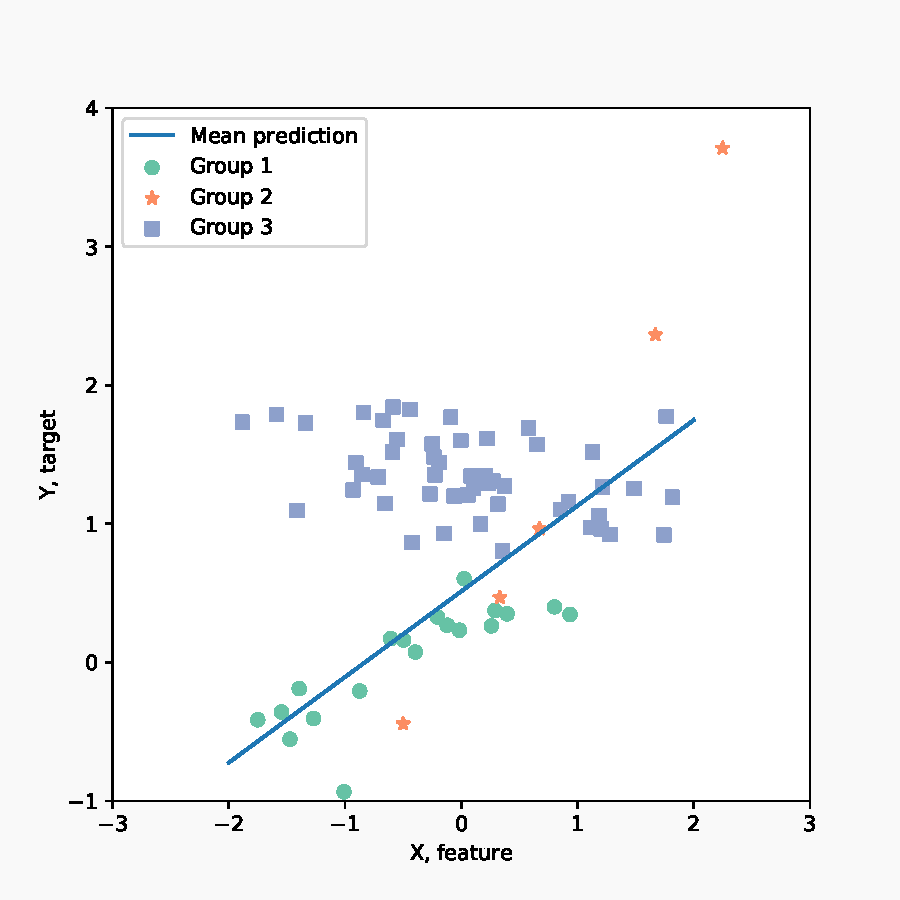
\includegraphics[width=0.9\textwidth]{Figures/lme_example_mean_prediction}
   	\end{figure}
   	\[
   		y = X\beta + \varepsilon, \quad \varepsilon \sim \NN(0, \Lambda) 
   	\]

   	
    \column{0.5\textwidth}
    	\centering  Linear Mixed-Effect Model:
   	\begin{figure}
   		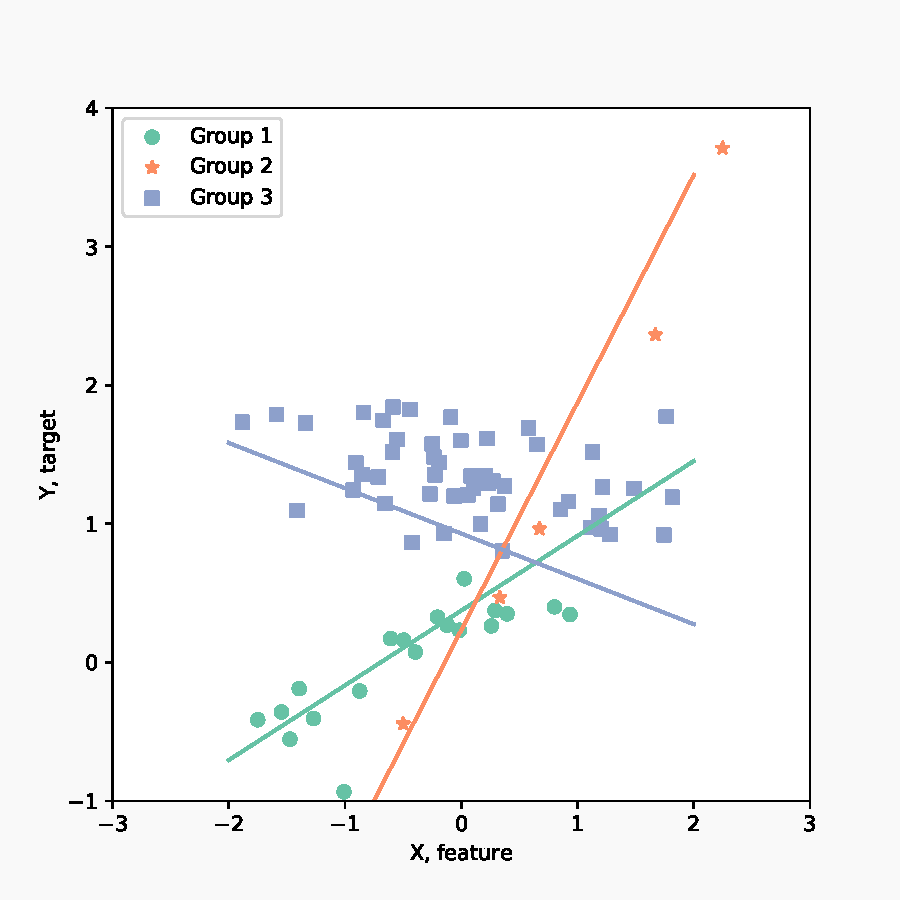
\includegraphics[width=0.9\textwidth]{Figures/lme_example_random_prediction}
   	\end{figure}
   	   		\[
   		\begin{split}
   			y_i & = X_i(\beta + {\color{red} u_i}) + \varepsilon_i, \quad \varepsilon_i \sim \NN(0, \Lambda_i) \\
   			{\color{red} u_i} & {\color{red}\sim \NN(0, \Gamma)}
   		\end{split}
   		\]

   	
  \end{columns}
\end{frame}

\begin{frame}{Notation}
	\eq{
   		y_i & = \alt<3->{X_i{\color<4,9>{red}\beta} + {\color<3>{red}Z_i}{\color<5,9>{red}u_i}}{{\color<2>{red}X_i}(\beta + u_i)} + \varepsilon_i \quad i = 1\dots m \\
   		{\color<7>{red}\varepsilon_i} & \sim \NN(0, {\color<8,9>{red}\Lambda_i}) \\
   		u_i & \sim \NN(0, {\color<6,9>{red}\Gamma})
   	}   	
   	
   	\begin{itemize}
   		\item<2-> $X_i \in \R^{n_i \times p}$ -- \only<3>{{\color{red} fixed}}\only<4->{fixed} features, or covariates, \only<3>{{\color{red} $Z_i \in \R^{n_i \times q}$ -- random features }}\only<4->{ $Z_i \in R^{n_i \times q}$ -- random features}
   		\item<3-> $p$ -- number of fixed features, $q$ -- number of random effects.
   		\item<4-> $\beta \in \R^p$ -- fixed effects, or mean effects
   		\item<5-> $u_i \in \R^q$ -- random effects
   		\item<6-> $\Gamma \in \R^{q \times q}$ -- covariance matrix of random effects
   		\item<7-> $\varepsilon_i \in \R^{n_i}$ -- observation noise
   		\item<8-> $\Lambda_i \in R^{n_i \times n_i}$ -- covariance matrix for noise
   		\item<9-> Unknowns: $\beta$, $u_i$, $\Gamma$, sometimes $\Lambda_i$.
   		
   	\end{itemize}
   	\uncover<10->{
   	\[
   		\Gamma = \diag{({\color{red}\gamma})},\ {\color{red}\gamma \in \R^{q}} \quad \text{ and } \Lambda_i \text{ are known.}
   	\]
   	}
\end{frame}

\begin{frame}[fragile]{Likelihood for Mixed Models}
Suppose we have a linear mixed effects model 

\eq{
	\label{eq:lmm_setup}
	Y_i & = X_i\beta + Z_iu_i + \varepsilon_i \\
	u_i & \sim \NN(0, \Gamma), \ \Gamma = \diag{\gamma} \\
	\varepsilon_i & \sim \NN(0, \Lambda_i)\\
}
where $\beta$, $\gamma$, and $u_i$ are unknown model parameters, and $\lambda_i$ are known.


	Noticing that $Z_iu_i + \varepsilon_i \sim \NN(0, Z_i\Gamma Z_i^T + \Lambda_i)$ we get the negative log-likelihood:
	 \eq{
	\label{eq:lmm_objective}
	\mathcal{L}(\beta, \gamma) & = \sum_{i = 1}^m \half(y_i - X_i\beta)^T(Z_i\Gamma Z_i^T + \Lambda_i)^{-1}(y_i - X_i\beta) + \\ & + \half\log{\det{\pa{Z_i \Gamma Z_i^T + \Lambda_i}}}
	}

\end{frame}
	
\subsection{Feature Selection for Mixed Models}
\begin{frame}{Feature Selection for Mixed Models}

Consider the following feature selection setup:

\eq{
	\min_{\beta, \gamma} & \LL(\beta, \gamma) \\
	\text{s.t. } & \|\beta\|_0 \leq k \\
	& \|\gamma\|_0 \leq j \\
	& \gamma \geq 0
}

where $k$ and $j$ is the size of the sparse support for the fixed and random effects respectively.

This is a very hard problem to solve directly.

\end{frame}

\begin{frame}{Methods for Feature Selection}
There are several ways to address this setup:
  \begin{columns}[T,onlytextwidth]
    \column{0.33\textwidth}
    (0) Exhaustive Search:
\[
	\begin{split}
	\min_{\beta, \gamma} & \LL(\beta, \gamma) \\
	\text{s.t. } & \|\beta\|_0 \leq k \\
	& \|\gamma\|_0 \leq j \\
	& \gamma \geq 0
	\end{split}
\]

    \column{0.33\textwidth}
    \uncover<2->{
    \centering
    (1) $\ell_1$-relaxation:
\[
	\begin{split}
	\min_{\beta, \gamma} & \LL(\beta, \gamma) \\
	\text{s.t. } & \|\beta\|_{\color{red}1} \leq {\color{red} \lambda_\beta} \\
	& \|\gamma\|_{\color{red}1} \leq {\color{red} \lambda_\gamma} \\
	& \gamma \geq 0
	\end{split}
\]
	}
	\column{0.33\textwidth}
	\uncover<3->{
    \centering
    (3) Other types of sparsity-inducing penalties\\ ($\ell_p$, $SCAD$).
    }
  \end{columns}
  
 \onslide<1-3>{
	\begin{columns}[T, onlytextwidth]
	\column{0.33\textwidth}
	\onslide<1-3>{
	\centering
	AIC \cite{Vaida2005}\\
	BIC \cite{Jones2011}\\
	}
	\column{0.33\textwidth}
	\onslide<2-3>{
	\centering
	M-ALASSO \cite{Bondell2010} \\
	ALASSO \cite{Lin2013} \\
	}
	\column{0.33\textwidth}
	\onslide<3>{
	\centering
	SCAD \cite{Fan2001}\\
	SCAD-P \cite{Fan2012}
	}
	\end{columns}
}

\onslide<4->{
	\begin{center}
	(2) SR3-type Relaxation \cite{Zheng2019}
	\eq{
	\min_{\beta, \gamma, {\color{red}\hbeta}, {\color{red}\tgamma}} & \LL(\beta, \gamma) + {\color{red}\frac{\lambda_\beta}{2}\|\beta - \tbeta\|^2_2 + \frac{\lambda_{\gamma}}{2}\|\gamma - \tgamma\|_2^2}\\
	\text{s.t. } 	& \|{\color{red}\tbeta}\|_0 \leq k \\
					& \|{\color{red}\tgamma}\|_0 \leq j, \  \gamma \geq 0
	}
	\end{center}
	}
  
 

\end{frame}
\section{Proposed Algorithm}
\begin{frame}{Relax-and-Split from Optimization Perspective}
\eq{
	{\color<2, 3>{red}\min}_{{\color<2>{red}\beta, \gamma,} {\color<3>{red}\tbeta, \tgamma}} & {\color<2>{red}\LL(\beta, \gamma)} + {\color<2,3>{red}\frac{{\color<4>{red}\lambda_\beta}}{2}\|\beta - \tbeta\|^2_2} + {\color<2,3>{red}\frac{{\color<4>{red}\lambda_\gamma}}{2}\|\gamma - \tgamma\|_2^2}\\
	\text{s.t. } 	& {\color<3>{red}\|\tbeta\|_0 \leq k, \ \|\tgamma\|_0 \leq j} \\ 
		& {\color<2>{red}\gamma \geq 0}, \ {\color<3>{red}\tgamma \geq 0}
	}
We'll find $\beta^*$, $\gamma^*$, $\tbeta^*$, and $\tgamma^*$ via alternating partial minimization:

\begin{itemize}
	\item<2-> Minimization w.r.t. $\beta$ and $\gamma$ is done via \textbf{Interior Point Method}.
	\item<3-> Minimization w.r.t. $\tbeta$ and $\tgamma$ is \textbf{projection} of $\beta$ and $\gamma$ onto $\ell_0$-balls.
	\item<4-> $\lambda_\beta$ and $\lambda_\gamma$ are \textbf{iteratively increased} until $\tbeta \approx \beta$ and $\tgamma \approx \gamma$.
\end{itemize}
\only<-4>{
\visible<3>{
	\eq{
		\tbeta^{(k+1)} \leftarrow \proj_{\|\beta\|_0 \leq k}(\beta^{(k)}) \quad &\implies \quad \text{Take max k from } \beta \text{, rest to 0} \\
		\tgamma^{(k+1)} \leftarrow \proj_{\|\gamma\|_0 \leq s}(\gamma^{(k)})\quad &\implies \quad \text{Take max j from }\gamma \text{, rest to 0}
		}
}
}
\only<5->{
\textbf{Advantages}:
\begin{enumerate}
	\item Interpretable hyperparameters.
	\item No model bias when the $k-$subspace is chosen.
\end{enumerate}
}
\end{frame}

%\begin{frame}{Interior Point Method}
%The Lagrangian of the barrier relaxation is:
%	\eq{
%	F_\mu(v, \beta, \gamma) & = \LL(\beta, \gamma) +  \frac{\lambda_\beta}{2}\|\beta - \tbeta^{(k)}\|^2_2 + \frac{\lambda_\gamma}{2}\|\gamma - \tgamma^{(k)}\|_2^2 + \\ & + \mu\sum_{i=1}^{q}\log(\gamma_i) - v^T\gamma \\
%	}
%	The descent direction is chosen as:
%	\eq{
%	\nabla^2F_\mu\begin{bmatrix}
%		\Delta v \\
%		\Delta \beta \\
%		\Delta \gamma
%	\end{bmatrix} = -\nabla F_\mu\begin{bmatrix}
%		\Delta v \\
%		\Delta \beta \\
%		\Delta \gamma
%	\end{bmatrix}
%	\text{, step is: }
%	\begin{cases}
%	v^{(k+1)} = v^{(k)} + \alpha_k \Delta v \\
%	\gamma^{(k+1)} = \gamma^{(k)} + \alpha_k \Delta\gamma \\
%	\beta^{(k+1)} = \beta^{(k)} + \alpha_k \Delta \beta
%	\end{cases}
%	}
%	and $\alpha_k$ is chosen such that
%	\eq{
%	& \gamma^{(k+1)} \geq 0,\ v^{(k+1)} \geq 0 \\
%	& \|\nabla F_\mu(v^{(k+1)}, \beta^{(k+1)}, \gamma^{(k+1)})\| \leq 0.99\|\nabla F_\mu(v^{(k)}, \beta^{(k)}, \gamma^{(k)})\| 
%	}
%\end{frame}

\begin{frame}{R\&S-Mixed}
The pseudocode of the proposed algorithm:
{\small
\begin{algorithm}[H]
	$\lambda_\beta = 0$; $\lambda_\gamma = 0$ \\
	\Repeat{$\tbeta \approx \beta, \tgamma \approx \gamma$}{
	$\lambda_\beta \leftarrow 2(1 + \lambda_\beta)$ \\
	$\lambda_\gamma \leftarrow 2(1 + \lambda_\gamma)$\\
	\Repeat{converges}{
		$\tbeta^{(k+1)} \leftarrow \proj_{\|\beta\|_0 \leq k}(\beta^{(k)})$\\ 
		$\tgamma^{(k+1)} \leftarrow \proj_{\|\gamma\|_0 \leq s}(\gamma^{(k)})$ \\
		$\beta^{(k+1)}, \gamma^{(k+1)} \leftarrow \argmin_{\gamma \geq 0, \beta}\LL(\beta, \gamma) + \frac{\lambda_\beta}{2}\|\beta - \tbeta^{(k)}\|^2_2 + \frac{\lambda_\gamma}{2}\|\gamma - \tgamma^{(k)}\|_2^2$
	}
	}
	\BlankLine
\end{algorithm}
	}
\end{frame}

\section{Experiments}
\subsection{Application to Synthetic Problems}

\begin{frame}{Performance in Comparison to Other Algorithms}
\begin{itemize}
	\item \textbf{Scenario 1}: $n=30$, $n_i=5$, $p = 9$, $q = 4$, with true parameters $\beta = (1, 1, 0, \dots, 0)$ and the covariance matrix $\Gamma$ being: 
		\eq{
			\Gamma = \begin{bmatrix}
				9 & 4.8 & 0.6 & 0 \\
				4.8 & 4 & 1 & 0 \\
				0.6 & 1 & 1 & 0\\
				0 & 0 & 0 & 0
			\end{bmatrix}
		}
	\item \textbf{Scenario 2}: everything as in Scenario 1, but $n=60$ and $n_i=10$.
\end{itemize}
\textbf{Competitors}:
\begin{itemize}
	\item \textbf{ALASSO:} 2 stage: A-LASSO+Newton and A-LASSO+PCO
	\item \textbf{M-ALASSO:} Adaptive LASSO + EM Algorithm
	\item \textbf{SCAD-P:} SCAD + Proxy Matrix for $\Gamma$
	\item \textbf{rPQL:} Quasi-Likelihood + Adaptive LASSO (for GLMMs)
\end{itemize}
\end{frame}

\begin{frame}{Performance in Comparison to Other Algorithms}
\begin{table}[H]
\begin{center}
\begin{tabular}{|l|l|c|c|c|c|c|}
\hline
Setup & Algoritm & \% C & \% CF & \% CR & MSE & TIME \\
\hline 
\hline
$n = 30$, $n_i = 5$ & \textbf{\ouralgo} & 58 & 72 & 78 & 0.66 & 0.015 \\
& rPQL & 88 & 98 & 88 & 0.88 & 26-59 \\ 
& M-ALASSO & 71 & 73 & 79 & - & -\\
& ALASSO & 79 & 81 & 96 & - & - \\
& SCAD-P & - & 90 & 86 & - & - \\
\hline 
$n = 60$, $n_i = 10$ & \textbf{\ouralgo} & 98 & 100  & 98 & 0.69& 0.018 \\
& rPQL & 98 & 99 & 98 & 0.97 &  26-59 \\ 
& M-ALASSO & 83 & 83 & 89 & - & - \\
& ALASSO & 95 & 96 & 99 & - & -\\
& SCAD-P & 100 & 100 & 100 & - & - \\
\hline
	
\end{tabular}
\end{center}
\caption{\label{table:krishna_setup_results} Comparison of feature selection algorithms. \% CF -- percent of models where true fixed effects were identified correctly, \% CR -- percent of models where true random effects were identified correctly, \% C -- both fixed and random effects were identified correctly.}	
\end{table}
	
\end{frame}

\begin{frame}{Scalability Experiment}
\begin{itemize}
	\item $n = 60$, $n_i = 10$
	\item $p = q \in [4, 7, 10, \dots, 90]$, 200 experiments for each.
	\item $X_i = Z_i$, columns are drawn form $\NN(0, \Psi)$ where
	\[
		\Psi = \begin{bmatrix}
			9 & 4.8 & 0.6 \\
			4.8 & 4 & 1 \\
			0.6 & 1 & 1 \\
		\end{bmatrix}
	\]
	\item 50\% random coordinate in $\beta$ are active
	\item 70\% of those are also active in $\gamma$
\end{itemize}
\end{frame}

\begin{frame}{Scalability Experiment}
		\begin{center}
			\includegraphics<+>[width=0.8\textwidth]{Figures/scalability_accuracy}
			%\includegraphics<+>[width=0.8\textwidth]{Figures/scalability_mse}
		\end{center}
\end{frame}

\subsection{Application to Real-World Problems}

\begin{frame}{Contact Rate Modeling for COVID-19 Forecasting}
	\begin{itemize}
		\item $n = 60$ groups (countries and US states), $n_i \approx 50$
		\item $Y_i$ -- contact rate for COVID SEIIR Model 
		\item $p=q=5$ covariates related to temperature, mobility, population, testing; plus intercept.
	\end{itemize}
\end{frame}

\begin{frame}{Contact Rate Modeling for COVID-19 Forecasting}
	\begin{center}
		\includegraphics<+>[width=\textwidth]{Figures/fit_Alaska}
		\includegraphics<+>[width=\textwidth]{Figures/fit_Slovenia}
		\includegraphics<+>[width=\textwidth]{Figures/fit_Switzerland}
		\includegraphics<+>[width=\textwidth]{Figures/fit_Turkey}
	\end{center}
\end{frame}

\begin{frame}{Burden of Anxiety and Depression as Result of Bullying}
	\begin{itemize}
		\item $m = 10$ cohort studies, $n = 77$, highly unbalanced 
		\item $p = 13$, $q = 12$ (\texttt{time} was preselected fixed-only)
		\item Covariates are related to studies' designs.
	\end{itemize}
\end{frame}

\begin{frame}{Burden of Anxiety and Depression as Result of Bullying}
	\begin{center}
		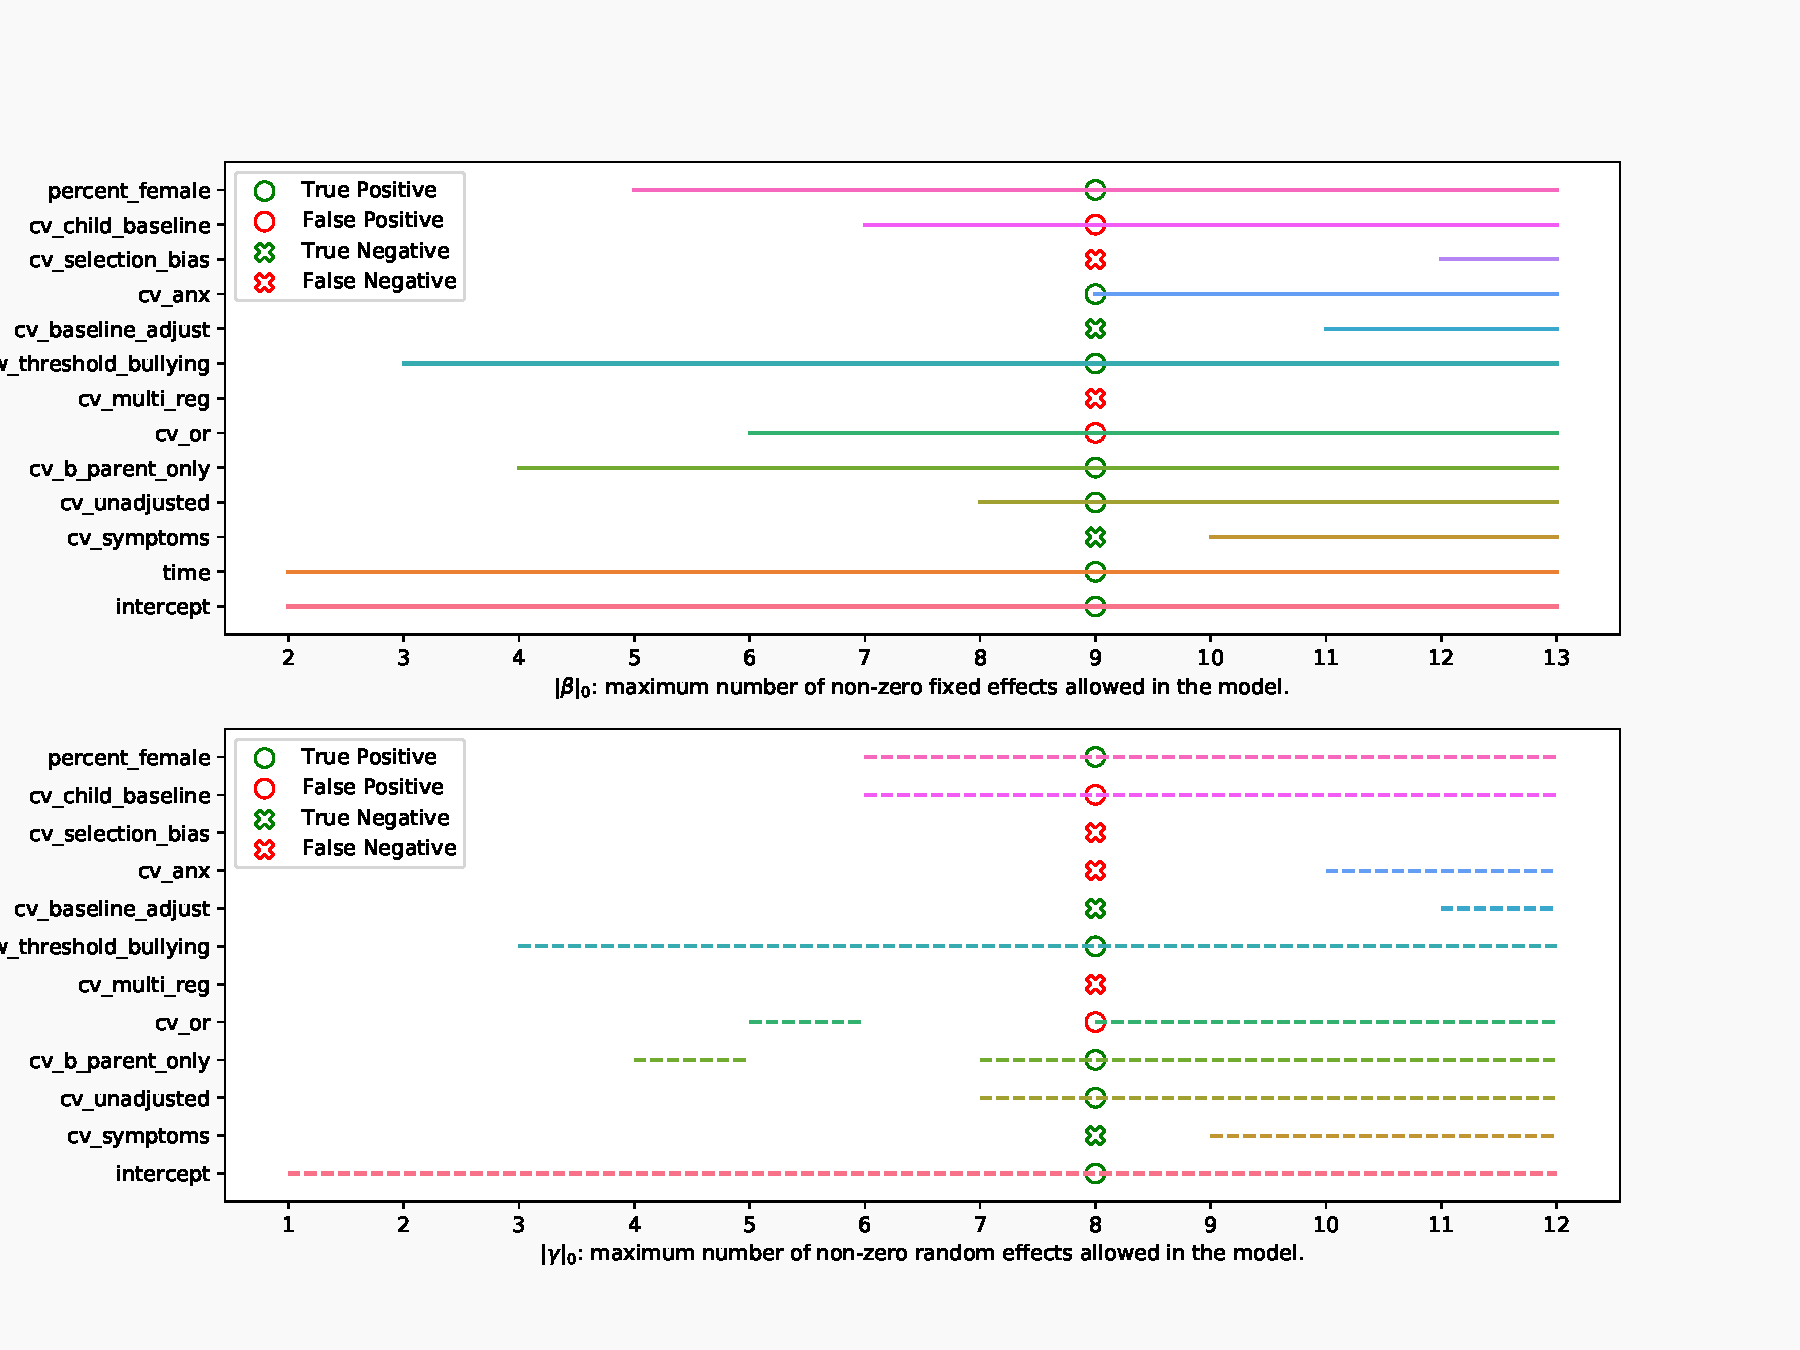
\includegraphics[width=\textwidth]{Figures/bullying_data.csv_inclusion}
		%\includegraphics<+>[width=\textwidth]{Figures/bullying_data.csv_fixed_feature_selection}
		%\includegraphics<+>[width=\textwidth]{Figures/bullying_data.csv_random_feature_selection}

	\end{center}
\end{frame}
\section{Future Work}
\begin{frame}{Future Work: Theory}
\begin{theorem}[Conditions for Convergence to True Estimator]
	Under certain conditions the method converges in a finite number of iterations to $(\hat\beta, \hat\gamma)$ which projections $(\tbeta, \tgamma)$ belong to a $k$- and $j$-subspaces respectively that contain the true minimum $(\beta^*,\gamma^*)$.
\end{theorem}
\begin{theorem}[Consistency of Estimator]
	There exists a local minimizer $(\hat{\beta}, \hat{\gamma})$ for the proposed loss function, such that it is asymptotically consistent with true minimum $(\beta^*, \gamma^*)$. 
\end{theorem}
\begin{theorem}[Consistency in Zeros]
	If some coordinates of the true minimizer ($\beta^*, \gamma^*$) are zero, then it is also zero in $(\hat{\beta}, \hat{\gamma})$, given that the later is sufficiently close to the former.
\end{theorem}
\begin{theorem}[Asymptotic Normality]
	The proposed estimator $(\hat{\beta}, \hat{\gamma})$ asymptotically normally distributed around true minimizer ($\beta^*, \gamma^*$) in its true non-zero $k+j$-subspace.
\end{theorem}	
\end{frame}

\begin{frame}{Future work: Algorithm}
	\textbf{Question:} Will exponential smoothing of projection improve the accuracy? 
	{\small
	\begin{algorithm}[H]
	$\lambda_\beta = 0$; $\lambda_\gamma = 0$ \\
	\Repeat{$\tbeta \approx \beta, \tgamma \approx \gamma$}{
	$\lambda_\beta \leftarrow 2(1 + \lambda_\beta)$ \\
	$\lambda_\gamma \leftarrow 2(1 + \lambda_\gamma)$\\
	\Repeat{converges}{
		$\tbeta^{(k+1)} \leftarrow {\color{red}\delta}\proj_{\|\beta\|_0 \leq k}(\beta^{(k)}) + {\color{red}(1-\delta)\tbeta^{(k)}}$\\
		$\tgamma^{(k+1)} \leftarrow {\color{red}\delta}\proj_{\|\gamma\|_0 \leq s}(\gamma^{(k)}) + {\color{red}(1-\delta)\tgamma^{(k)}}$\\
		$\beta^{(k+1)}, \gamma^{(k+1)} \leftarrow \argmin_{\gamma \geq 0, \beta}\LL(\beta, \gamma) + \frac{\lambda_\beta}{2}\|\beta - \tbeta^{(k)}\|^2_2 + \frac{\lambda_\gamma}{2}\|\gamma - \tgamma^{(k)}\|_2^2$
	}
	}
	\BlankLine
	\end{algorithm}
	}
	\end{frame}
	
\begin{frame}{Future Work: Implementation}
		Can we increase $\lambda_\beta$ and $\lambda_\gamma$ in a more careful way to avoid potential stacking? 
		The approach can be based on the theorem:
		\begin{theorem}[Distance Between Minima]
	For a fixed dataset $(X_i, Y_i)$ and relaxation parameters $\lambda_\beta$, $\lambda_\gamma$ the distance between $(\beta^*, \gamma^*)$, the unconstrained minimizers of relaxed problem, and their projections $(\tbeta^*, \tgamma^*)$ is bounded by a constant $M$ depending on $(X_i, Y_i)$ and the relaxation parameters.
		\end{theorem}
\end{frame}

\begin{frame}{The End}
	\begin{center}
		\large Thank you for your attention!
	\end{center}
\end{frame}


\begin{frame}[allowframebreaks]{References}

  \bibliography{bibliography}
  \bibliographystyle{alpha}

\end{frame}

\end{document}